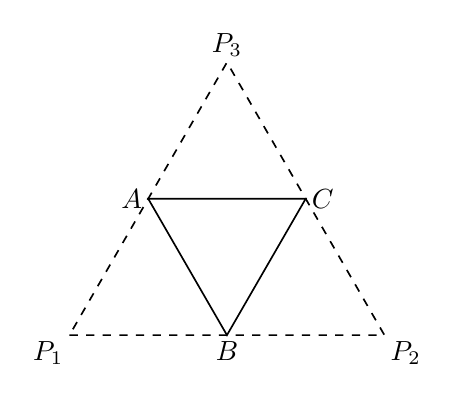
\begin{tikzpicture}[x=1cm,y=1cm,font=\normalsize,
 geometry edge/.style={solid,line width=.6pt},
 geometry mark/.style={solid,line width=.6pt},
 geometry label/.style={font=\normalsize,inner sep=2pt}]
\coordinate (P1) at (0.0000,0.0000);
\coordinate (P2) at (4.0000,0.0000);
\coordinate (P3) at (2.0000,3.4641);
\coordinate (A) at (1.0000,1.7321);
\coordinate (B) at (2.0000,0.0000);
\coordinate (C) at (3.0000,1.7321);
\draw[geometry edge,dashed] (P1)--(P2)--(P3)--cycle;
\draw[geometry edge] (A)--(B)--(C)--cycle;
\node[geometry label,below left] at (P1) {$P_1$};
\node[geometry label,below right] at (P2) {$P_2$};
\node[geometry label,above] at (P3) {$P_3$};
\node[geometry label,left] at (A) {$A$};
\node[geometry label,below] at (B) {$B$};
\node[geometry label,right] at (C) {$C$};
\end{tikzpicture}
